%\title{Escher Illusions in LaTeX}
% Author: Julien Cretel
% Date:   24/02/2013
% From: http://www.texample.net/tikz/examples/escher-brick-penrose-triangle/
\documentclass{article}
\usepackage{tikz}

\begin{document}


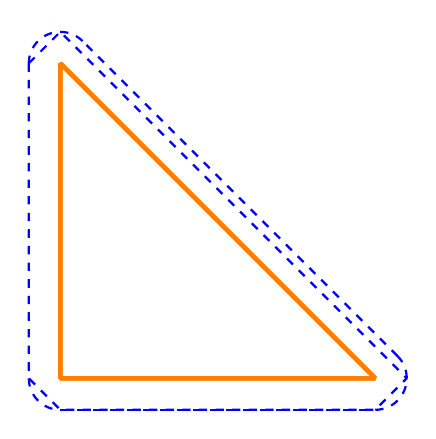
\begin{tikzpicture}[scale=4, line join=bevel]

\draw[orange, ultra thick] (0,0) -- (1,0) -- (0,1) -- cycle;
\draw[blue, thick, dashed] (-0.1,1) -- (-0.1,0);
\draw[blue, thick, dashed] (-0.1,0) arc (180:270:0.1);
\draw[blue, thick, dashed] (0,-0.1) -- (1,-0.1);
\draw[blue, thick, dashed] (1,-0.1) arc (-90:45:0.1);
\draw[blue, thick, dashed] (1.0707, 0.0707) --  (0.0707,1.0707); 
\draw[blue, thick, dashed] (0.0707,1.0707) arc (45:180:0.1);


\draw[orange, ultra thick] (0,0) -- (1,0) -- (0,1) -- cycle;
\draw[blue, thick, dashed] (-0.1,1) -- (-0.1,0) --
 (-0.1,0) -- (0,-0.1)--
  (0,-0.1) -- (1,-0.1)-- 
  (1.1, 0) --  (0,1.1)  -- cycle;; 

\end{tikzpicture}

\skip

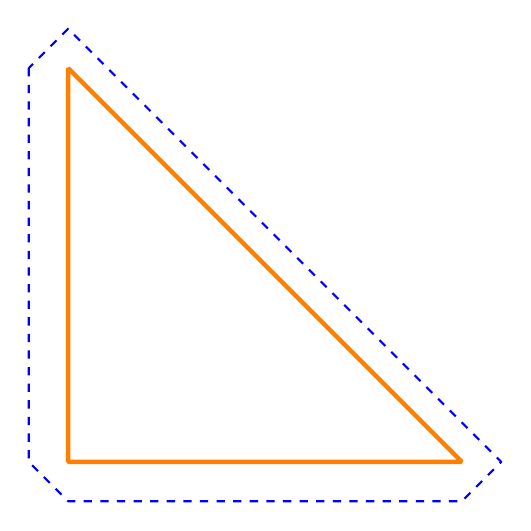
\begin{tikzpicture}[scale=5, line join=bevel]
\draw[orange, ultra thick] (0,0) -- (1,0) -- (0,1) -- cycle;
\draw[blue, thick, dashed] (-0.1,1) -- (-0.1,0) --
 (-0.1,0) -- (0,-0.1)--
  (0,-0.1) -- (1,-0.1)-- 
  (1.1, 0) --  (0,1.1)  -- cycle;; 



\end{tikzpicture}

\end{document}
